\documentclass[14pt]{extbook}
\usepackage{multicol, enumerate, enumitem, hyperref, color, soul, setspace, parskip, fancyhdr} %General Packages
\usepackage{amssymb, amsthm, amsmath, latexsym, units, mathtools} %Math Packages
\everymath{\displaystyle} %All math in Display Style
% Packages with additional options
\usepackage[headsep=0.5cm,headheight=12pt, left=1 in,right= 1 in,top= 1 in,bottom= 1 in]{geometry}
\usepackage[usenames,dvipsnames]{xcolor}
\usepackage{dashrule}  % Package to use the command below to create lines between items
\newcommand{\litem}[1]{\item#1\hspace*{-1cm}\rule{\textwidth}{0.4pt}}
\pagestyle{fancy}
\lhead{Progress Quiz 5}
\chead{}
\rhead{Version ALL}
\lfoot{8497-6012}
\cfoot{}
\rfoot{Summer C 2021}
\begin{document}

\begin{enumerate}
\litem{
Determine the vertical asymptotes and holes in the rational function below.\[ f(x) = \frac{4x^{3} +4 x^{2} -33 x -45}{6x^{2} -x -15} \]\begin{enumerate}[label=\Alph*.]
\item \( \text{Vertical Asymptote of } x = 1.667 \text{ and hole at } x = -1.5 \)
\item \( \text{Vertical Asymptote of } x = 0.667 \text{ and hole at } x = -1.5 \)
\item \( \text{Vertical Asymptotes of } x = 1.667 \text{ and } x = -1.5 \text{ with no holes.} \)
\item \( \text{Vertical Asymptotes of } x = 1.667 \text{ and } x = -2.5 \text{ with a hole at } x = -1.5 \)
\item \( \text{Holes at } x = 1.667 \text{ and } x = -1.5 \text{ with no vertical asymptotes.} \)

\end{enumerate} }
\litem{
Determine the vertical asymptotes and holes in the rational function below.\[ f(x) = \frac{12x^{3} +59 x^{2} +29 x -60}{12x^{2} +35 x + 25} \]\begin{enumerate}[label=\Alph*.]
\item \( \text{Vertical Asymptote of } x = -1.25 \text{ and hole at } x = -1.667 \)
\item \( \text{Holes at } x = -1.25 \text{ and } x = -1.667 \text{ with no vertical asymptotes.} \)
\item \( \text{Vertical Asymptote of } x = 1.0 \text{ and hole at } x = -1.667 \)
\item \( \text{Vertical Asymptotes of } x = -1.25 \text{ and } x = -1.667 \text{ with no holes.} \)
\item \( \text{Vertical Asymptotes of } x = -1.25 \text{ and } x = 0.75 \text{ with a hole at } x = -1.667 \)

\end{enumerate} }
\litem{
Determine the vertical asymptotes and holes in the rational function below.\[ f(x) = \frac{9x^{3} -15 x^{2} -2 x + 8}{6x^{2} +19 x + 10} \]\begin{enumerate}[label=\Alph*.]
\item \( \text{Vertical Asymptotes of } x = -2.5 \text{ and } x = -0.667 \text{ with no holes.} \)
\item \( \text{Vertical Asymptotes of } x = -2.5 \text{ and } x = 1.333 \text{ with a hole at } x = -0.667 \)
\item \( \text{Vertical Asymptote of } x = 1.5 \text{ and hole at } x = -0.667 \)
\item \( \text{Vertical Asymptote of } x = -2.5 \text{ and hole at } x = -0.667 \)
\item \( \text{Holes at } x = -2.5 \text{ and } x = -0.667 \text{ with no vertical asymptotes.} \)

\end{enumerate} }
\litem{
Determine the vertical asymptotes and holes in the rational function below.\[ f(x) = \frac{8x^{3} -2 x^{2} -43 x + 30}{6x^{2} +7 x -20} \]\begin{enumerate}[label=\Alph*.]
\item \( \text{Holes at } x = 1.333 \text{ and } x = -2.5 \text{ with no vertical asymptotes.} \)
\item \( \text{Vertical Asymptote of } x = 1.333 \text{ and hole at } x = -2.5 \)
\item \( \text{Vertical Asymptote of } x = 1.333 \text{ and hole at } x = -2.5 \)
\item \( \text{Vertical Asymptotes of } x = 1.333 \text{ and } x = 0.75 \text{ with a hole at } x = -2.5 \)
\item \( \text{Vertical Asymptotes of } x = 1.333 \text{ and } x = -2.5 \text{ with no holes.} \)

\end{enumerate} }
\litem{
Determine the horizontal and/or oblique asymptotes in the rational function below.\[ f(x) = \frac{8x^{3} -46 x^{2} +85 x -50}{4x^{2} +7 x -15} \]\begin{enumerate}[label=\Alph*.]
\item \( \text{Horizontal Asymptote of } y = -3.0 \text{ and Oblique Asymptote of } y = 2x -15 \)
\item \( \text{Horizontal Asymptote of } y = 2.0  \)
\item \( \text{Oblique Asymptote of } y = 2x -15. \)
\item \( \text{Horizontal Asymptote of } y = 2.0 \text{ and Oblique Asymptote of } y = 2x -15 \)
\item \( \text{Horizontal Asymptote at } y = -3.0 \)

\end{enumerate} }
\litem{
Determine the horizontal and/or oblique asymptotes in the rational function below.\[ f(x) = \frac{12x^{3} +11 x^{2} -45 x -50}{8x^{3} +28 x^{2} -26 x -20} \]\begin{enumerate}[label=\Alph*.]
\item \( \text{Horizontal Asymptote of } y = 0  \)
\item \( \text{Vertical Asymptote of } y = -1.000  \)
\item \( \text{None of the above} \)
\item \( \text{Vertical Asymptote of } y = 2  \)
\item \( \text{Horizontal Asymptote of } y = 1.500  \)

\end{enumerate} }
\litem{
Which of the following functions \textit{could} be the graph below?
\begin{center}
    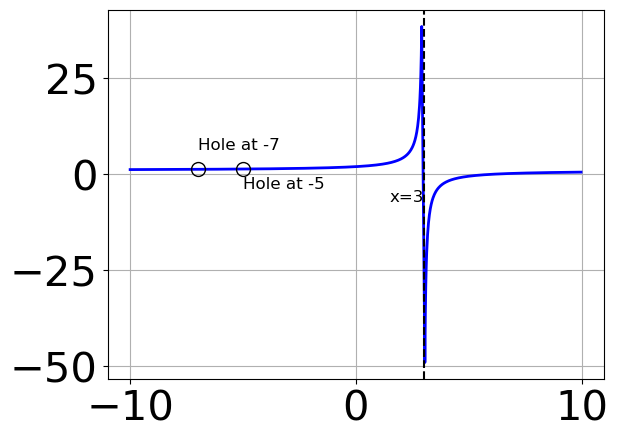
\includegraphics[width=0.5\textwidth]{../Figures/identifyGraphOfRationalFunctionCopyA.png}
\end{center}
\begin{enumerate}[label=\Alph*.]
\item \( f(x)=\frac{x^{3} +9.0 x^{2} -108.0}{x^{3} -9.0 x^{2} -x + 105.0} \)
\item \( f(x)=\frac{x^{3} +3.0 x^{2} -36.0 x -108.0}{x^{3} +9.0 x^{2} -x -105.0} \)
\item \( f(x)=\frac{x^{3} +6.0 x^{2} -37.0 x -210.0}{x^{3} +9.0 x^{2} -x -105.0} \)
\item \( f(x)=\frac{x^{3} -6.0 x^{2} -37.0 x + 210.0}{x^{3} -9.0 x^{2} -x + 105.0} \)
\item \( \text{None of the above are possible equations for the graph.} \)

\end{enumerate} }
\litem{
Determine the horizontal and/or oblique asymptotes in the rational function below.\[ f(x) = \frac{2x^{2} -3 x -9}{8x^{3} +22 x^{2} +3 x -18} \]\begin{enumerate}[label=\Alph*.]
\item \( \text{Horizontal Asymptote of } y = 0 \)
\item \( \text{Horizontal Asymptote at } y = 3.000 \)
\item \( \text{Horizontal Asymptote of } y = 0.250 \text{ and Oblique Asymptote of } y = 4x + 17 \)
\item \( \text{Oblique Asymptote of } y = 4x + 17. \)
\item \( \text{Horizontal Asymptote of } y = 0.250  \)

\end{enumerate} }
\litem{
Which of the following functions \textit{could} be the graph below?
\begin{center}
    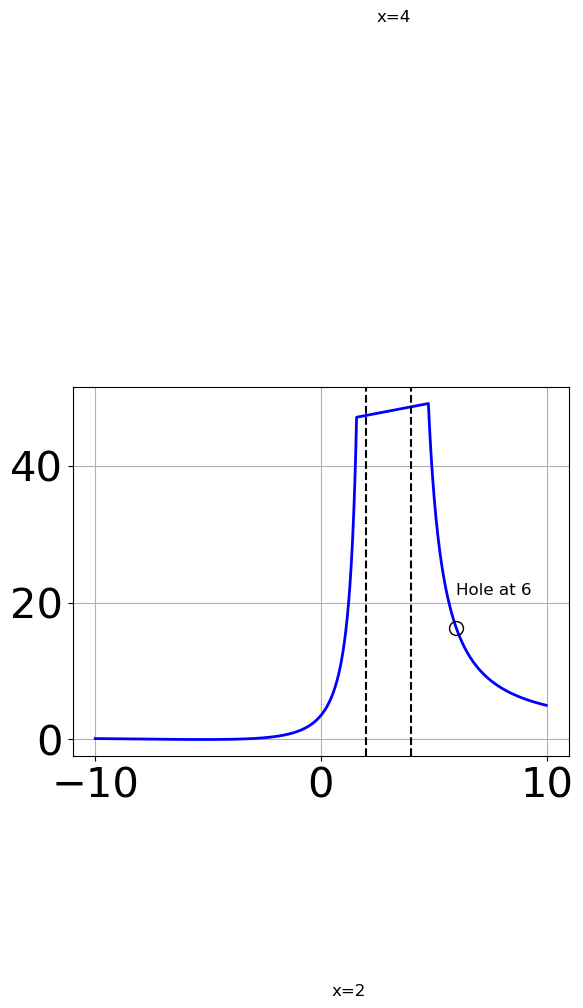
\includegraphics[width=0.5\textwidth]{../Figures/identifyGraphOfRationalFunctionA.png}
\end{center}
\begin{enumerate}[label=\Alph*.]
\item \( f(x)=\frac{x^{3} +5.0 x^{2} -38.0 x -168.0}{x^{3} -12.0 x^{2} +44.0 x -48.0} \)
\item \( f(x)=\frac{x^{3} -5.0 x^{2} -38.0 x + 168.0}{x^{3} +12.0 x^{2} +44.0 x + 48.0} \)
\item \( f(x)=\frac{x^{3} -4.0 x^{2} -49.0 x + 196.0}{x^{3} +12.0 x^{2} +44.0 x + 48.0} \)
\item \( f(x)=\frac{x^{3} +18.0 x^{2} +105.0 x + 196.0}{x^{3} -12.0 x^{2} +44.0 x -48.0} \)
\item \( \text{None of the above are possible equations for the graph.} \)

\end{enumerate} }
\litem{
Determine the horizontal and/or oblique asymptotes in the rational function below.\[ f(x) = \frac{6x^{3} +31 x^{2} +45 x + 18}{2x^{2} +13 x + 15} \]\begin{enumerate}[label=\Alph*.]
\item \( \text{Horizontal Asymptote of } y = 3.0 \text{ and Oblique Asymptote of } y = 3x -4 \)
\item \( \text{Horizontal Asymptote at } y = -5.0 \)
\item \( \text{Horizontal Asymptote of } y = -5.0 \text{ and Oblique Asymptote of } y = 3x -4 \)
\item \( \text{Horizontal Asymptote of } y = 3.0  \)
\item \( \text{Oblique Asymptote of } y = 3x -4. \)

\end{enumerate} }
\litem{
Determine the vertical asymptotes and holes in the rational function below.\[ f(x) = \frac{12x^{3} +83 x^{2} +165 x + 100}{6x^{2} +19 x + 15} \]\begin{enumerate}[label=\Alph*.]
\item \( \text{Holes at } x = -1.5 \text{ and } x = -1.667 \text{ with no vertical asymptotes.} \)
\item \( \text{Vertical Asymptotes of } x = -1.5 \text{ and } x = -1.667 \text{ with no holes.} \)
\item \( \text{Vertical Asymptote of } x = -1.5 \text{ and hole at } x = -1.667 \)
\item \( \text{Vertical Asymptote of } x = 2.0 \text{ and hole at } x = -1.667 \)
\item \( \text{Vertical Asymptotes of } x = -1.5 \text{ and } x = -1.25 \text{ with a hole at } x = -1.667 \)

\end{enumerate} }
\litem{
Determine the vertical asymptotes and holes in the rational function below.\[ f(x) = \frac{12x^{3} -41 x^{2} -40 x + 48}{12x^{2} -x -6} \]\begin{enumerate}[label=\Alph*.]
\item \( \text{Holes at } x = -0.667 \text{ and } x = 0.75 \text{ with no vertical asymptotes.} \)
\item \( \text{Vertical Asymptotes of } x = -0.667 \text{ and } x = 0.75 \text{ with no holes.} \)
\item \( \text{Vertical Asymptotes of } x = -0.667 \text{ and } x = -1.333 \text{ with a hole at } x = 0.75 \)
\item \( \text{Vertical Asymptote of } x = -0.667 \text{ and hole at } x = 0.75 \)
\item \( \text{Vertical Asymptote of } x = 1.0 \text{ and hole at } x = 0.75 \)

\end{enumerate} }
\litem{
Determine the vertical asymptotes and holes in the rational function below.\[ f(x) = \frac{6x^{3} -5 x^{2} -33 x -18}{6x^{2} +x -12} \]\begin{enumerate}[label=\Alph*.]
\item \( \text{Vertical Asymptote of } x = 1.333 \text{ and hole at } x = -1.5 \)
\item \( \text{Holes at } x = 1.333 \text{ and } x = -1.5 \text{ with no vertical asymptotes.} \)
\item \( \text{Vertical Asymptote of } x = 1.0 \text{ and hole at } x = -1.5 \)
\item \( \text{Vertical Asymptotes of } x = 1.333 \text{ and } x = -1.5 \text{ with no holes.} \)
\item \( \text{Vertical Asymptotes of } x = 1.333 \text{ and } x = -0.667 \text{ with a hole at } x = -1.5 \)

\end{enumerate} }
\litem{
Determine the vertical asymptotes and holes in the rational function below.\[ f(x) = \frac{4x^{3} +8 x^{2} -27 x -45}{8x^{2} +2 x -15} \]\begin{enumerate}[label=\Alph*.]
\item \( \text{Vertical Asymptotes of } x = 1.25 \text{ and } x = 2.5 \text{ with a hole at } x = -1.5 \)
\item \( \text{Vertical Asymptotes of } x = 1.25 \text{ and } x = -1.5 \text{ with no holes.} \)
\item \( \text{Holes at } x = 1.25 \text{ and } x = -1.5 \text{ with no vertical asymptotes.} \)
\item \( \text{Vertical Asymptote of } x = 0.5 \text{ and hole at } x = -1.5 \)
\item \( \text{Vertical Asymptote of } x = 1.25 \text{ and hole at } x = -1.5 \)

\end{enumerate} }
\litem{
Determine the horizontal and/or oblique asymptotes in the rational function below.\[ f(x) = \frac{6x^{3} + x^{2} -42 x -45}{3x^{2} +20 x + 25} \]\begin{enumerate}[label=\Alph*.]
\item \( \text{Horizontal Asymptote of } y = -5.0 \text{ and Oblique Asymptote of } y = 2x -13 \)
\item \( \text{Oblique Asymptote of } y = 2x -13. \)
\item \( \text{Horizontal Asymptote at } y = -5.0 \)
\item \( \text{Horizontal Asymptote of } y = 2.0 \text{ and Oblique Asymptote of } y = 2x -13 \)
\item \( \text{Horizontal Asymptote of } y = 2.0  \)

\end{enumerate} }
\litem{
Determine the horizontal and/or oblique asymptotes in the rational function below.\[ f(x) = \frac{6x^{2} -23 x + 15}{24x^{3} -134 x^{2} +167 x -60} \]\begin{enumerate}[label=\Alph*.]
\item \( \text{Horizontal Asymptote of } y = 0.250  \)
\item \( \text{Oblique Asymptote of } y = 4x -7. \)
\item \( \text{Horizontal Asymptote of } y = 0 \)
\item \( \text{Horizontal Asymptote at } y = 3.000 \)
\item \( \text{Horizontal Asymptote of } y = 0.250 \text{ and Oblique Asymptote of } y = 4x -7 \)

\end{enumerate} }
\litem{
Which of the following functions \textit{could} be the graph below?
\begin{center}
    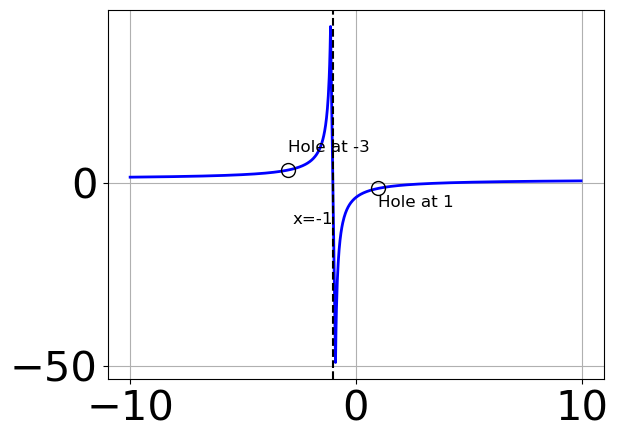
\includegraphics[width=0.5\textwidth]{../Figures/identifyGraphOfRationalFunctionCopyB.png}
\end{center}
\begin{enumerate}[label=\Alph*.]
\item \( f(x)=\frac{x^{3} +6.0 x^{2} -32.0}{x^{3} -3.0 x^{2} -x + 3.0} \)
\item \( f(x)=\frac{x^{3} +2.0 x^{2} -11.0 x -12.0}{x^{3} -3.0 x^{2} -x + 3.0} \)
\item \( f(x)=\frac{x^{3} -2.0 x^{2} -11.0 x + 12.0}{x^{3} +3.0 x^{2} -x -3.0} \)
\item \( f(x)=\frac{x^{3} -4.0 x^{2} -36.0 x + 144.0}{x^{3} +3.0 x^{2} -x -3.0} \)
\item \( \text{None of the above are possible equations for the graph.} \)

\end{enumerate} }
\litem{
Determine the horizontal and/or oblique asymptotes in the rational function below.\[ f(x) = \frac{6x^{2} -25 x -25}{12x^{3} +40 x^{2} -47 x -60} \]\begin{enumerate}[label=\Alph*.]
\item \( \text{Oblique Asymptote of } y = 2x + 15. \)
\item \( \text{Horizontal Asymptote of } y = 0 \)
\item \( \text{Horizontal Asymptote at } y = 5.000 \)
\item \( \text{Horizontal Asymptote of } y = 0.500  \)
\item \( \text{Horizontal Asymptote of } y = 0.500 \text{ and Oblique Asymptote of } y = 2x + 15 \)

\end{enumerate} }
\litem{
Which of the following functions \textit{could} be the graph below?
\begin{center}
    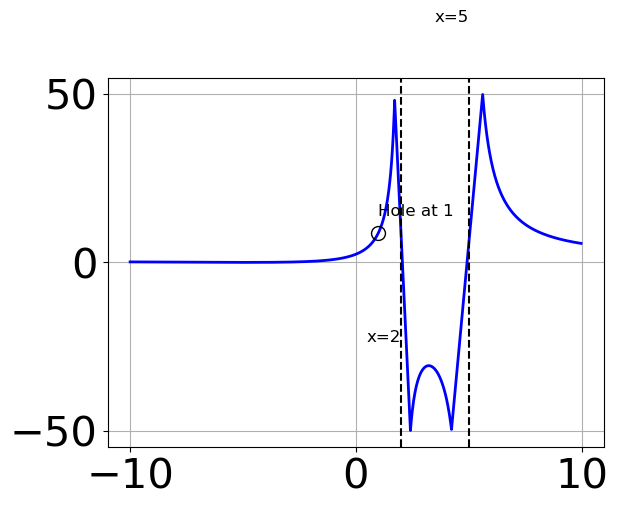
\includegraphics[width=0.5\textwidth]{../Figures/identifyGraphOfRationalFunctionB.png}
\end{center}
\begin{enumerate}[label=\Alph*.]
\item \( f(x)=\frac{x^{3} -9.0 x^{2} +14.0 x + 24.0}{x^{3} +8.0 x^{2} +17.0 x + 10.0} \)
\item \( f(x)=\frac{x^{3} -12.0 x^{2} +44.0 x -48.0}{x^{3} +8.0 x^{2} +17.0 x + 10.0} \)
\item \( f(x)=\frac{x^{3} +15.0 x^{2} +74.0 x + 120.0}{x^{3} -8.0 x^{2} +17.0 x -10.0} \)
\item \( f(x)=\frac{x^{3} +9.0 x^{2} +14.0 x -24.0}{x^{3} -8.0 x^{2} +17.0 x -10.0} \)
\item \( \text{None of the above are possible equations for the graph.} \)

\end{enumerate} }
\litem{
Determine the horizontal and/or oblique asymptotes in the rational function below.\[ f(x) = \frac{8x^{3} +10 x^{2} -13 x -15}{4x^{2} -21 x + 20} \]\begin{enumerate}[label=\Alph*.]
\item \( \text{Horizontal Asymptote of } y = 4.0 \text{ and Oblique Asymptote of } y = 2x + 13 \)
\item \( \text{Horizontal Asymptote of } y = 2.0 \text{ and Oblique Asymptote of } y = 2x + 13 \)
\item \( \text{Horizontal Asymptote at } y = 4.0 \)
\item \( \text{Oblique Asymptote of } y = 2x + 13. \)
\item \( \text{Horizontal Asymptote of } y = 2.0  \)

\end{enumerate} }
\litem{
Determine the vertical asymptotes and holes in the rational function below.\[ f(x) = \frac{8x^{3} +26 x^{2} -33 x -36}{16x^{2} -8 x -15} \]\begin{enumerate}[label=\Alph*.]
\item \( \text{Vertical Asymptotes of } x = 1.25 \text{ and } x = -0.75 \text{ with no holes.} \)
\item \( \text{Vertical Asymptotes of } x = 1.25 \text{ and } x = 1.5 \text{ with a hole at } x = -0.75 \)
\item \( \text{Vertical Asymptote of } x = 0.5 \text{ and hole at } x = -0.75 \)
\item \( \text{Holes at } x = 1.25 \text{ and } x = -0.75 \text{ with no vertical asymptotes.} \)
\item \( \text{Vertical Asymptote of } x = 1.25 \text{ and hole at } x = -0.75 \)

\end{enumerate} }
\litem{
Determine the vertical asymptotes and holes in the rational function below.\[ f(x) = \frac{12x^{3} +11 x^{2} -45 x -50}{6x^{2} +x -15} \]\begin{enumerate}[label=\Alph*.]
\item \( \text{Holes at } x = 1.5 \text{ and } x = -1.667 \text{ with no vertical asymptotes.} \)
\item \( \text{Vertical Asymptote of } x = 1.5 \text{ and hole at } x = -1.667 \)
\item \( \text{Vertical Asymptotes of } x = 1.5 \text{ and } x = -1.667 \text{ with no holes.} \)
\item \( \text{Vertical Asymptote of } x = 2.0 \text{ and hole at } x = -1.667 \)
\item \( \text{Vertical Asymptotes of } x = 1.5 \text{ and } x = -1.25 \text{ with a hole at } x = -1.667 \)

\end{enumerate} }
\litem{
Determine the vertical asymptotes and holes in the rational function below.\[ f(x) = \frac{12x^{3} +17 x^{2} -14 x -15}{12x^{2} +x -6} \]\begin{enumerate}[label=\Alph*.]
\item \( \text{Vertical Asymptotes of } x = 0.667 \text{ and } x = -0.75 \text{ with no holes.} \)
\item \( \text{Vertical Asymptote of } x = 1.0 \text{ and hole at } x = -0.75 \)
\item \( \text{Vertical Asymptote of } x = 0.667 \text{ and hole at } x = -0.75 \)
\item \( \text{Vertical Asymptotes of } x = 0.667 \text{ and } x = -1.667 \text{ with a hole at } x = -0.75 \)
\item \( \text{Holes at } x = 0.667 \text{ and } x = -0.75 \text{ with no vertical asymptotes.} \)

\end{enumerate} }
\litem{
Determine the vertical asymptotes and holes in the rational function below.\[ f(x) = \frac{8x^{3} +18 x^{2} -15 x -25}{12x^{2} -31 x + 20} \]\begin{enumerate}[label=\Alph*.]
\item \( \text{Vertical Asymptotes of } x = 1.333 \text{ and } x = -2.5 \text{ with a hole at } x = 1.25 \)
\item \( \text{Vertical Asymptotes of } x = 1.333 \text{ and } x = 1.25 \text{ with no holes.} \)
\item \( \text{Holes at } x = 1.333 \text{ and } x = 1.25 \text{ with no vertical asymptotes.} \)
\item \( \text{Vertical Asymptote of } x = 0.667 \text{ and hole at } x = 1.25 \)
\item \( \text{Vertical Asymptote of } x = 1.333 \text{ and hole at } x = 1.25 \)

\end{enumerate} }
\litem{
Determine the horizontal and/or oblique asymptotes in the rational function below.\[ f(x) = \frac{12x^{3} +25 x^{2} -4 x -12}{4x^{2} +23 x + 15} \]\begin{enumerate}[label=\Alph*.]
\item \( \text{Oblique Asymptote of } y = 3x -11. \)
\item \( \text{Horizontal Asymptote of } y = 3.0  \)
\item \( \text{Horizontal Asymptote of } y = 3.0 \text{ and Oblique Asymptote of } y = 3x -11 \)
\item \( \text{Horizontal Asymptote of } y = -5.0 \text{ and Oblique Asymptote of } y = 3x -11 \)
\item \( \text{Horizontal Asymptote at } y = -5.0 \)

\end{enumerate} }
\litem{
Determine the horizontal and/or oblique asymptotes in the rational function below.\[ f(x) = \frac{12x^{3} +83 x^{2} +165 x + 100}{3x^{3} -5 x^{2} -65 x -100} \]\begin{enumerate}[label=\Alph*.]
\item \( \text{Vertical Asymptote of } y = -4  \)
\item \( \text{None of the above} \)
\item \( \text{Horizontal Asymptote of } y = 0  \)
\item \( \text{Horizontal Asymptote of } y = 4.000  \)
\item \( \text{Vertical Asymptote of } y = 5.000  \)

\end{enumerate} }
\litem{
Which of the following functions \textit{could} be the graph below?
\begin{center}
    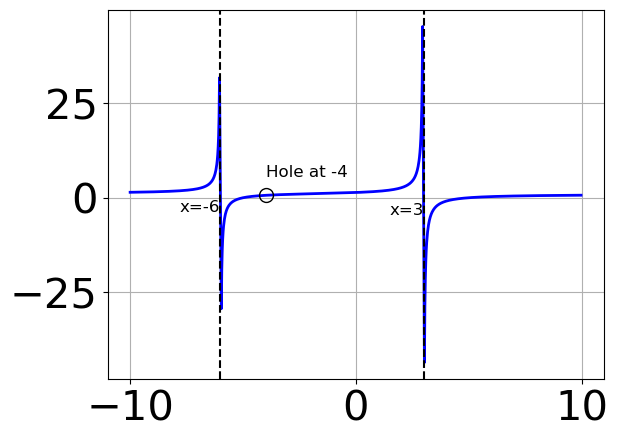
\includegraphics[width=0.5\textwidth]{../Figures/identifyGraphOfRationalFunctionCopyC.png}
\end{center}
\begin{enumerate}[label=\Alph*.]
\item \( f(x)=\frac{x^{3} -5.0 x^{2} -25.0 x + 125.0}{x^{3} -7.0 x^{2} -6.0 x + 72.0} \)
\item \( f(x)=\frac{x^{3} -5.0 x^{2} -25.0 x + 125.0}{x^{3} +7.0 x^{2} -6.0 x -72.0} \)
\item \( f(x)=\frac{x^{3} +4.0 x^{2} -25.0 x -100.0}{x^{3} +7.0 x^{2} -6.0 x -72.0} \)
\item \( f(x)=\frac{x^{3} -4.0 x^{2} -25.0 x + 100.0}{x^{3} -7.0 x^{2} -6.0 x + 72.0} \)
\item \( \text{None of the above are possible equations for the graph.} \)

\end{enumerate} }
\litem{
Determine the horizontal and/or oblique asymptotes in the rational function below.\[ f(x) = \frac{5x^{2} +27 x + 10}{15x^{3} + x^{2} -12 x -4} \]\begin{enumerate}[label=\Alph*.]
\item \( \text{Horizontal Asymptote of } y = 0.333 \text{ and Oblique Asymptote of } y = 3x -16 \)
\item \( \text{Horizontal Asymptote at } y = -5.000 \)
\item \( \text{Horizontal Asymptote of } y = 0 \)
\item \( \text{Oblique Asymptote of } y = 3x -16. \)
\item \( \text{Horizontal Asymptote of } y = 0.333  \)

\end{enumerate} }
\litem{
Which of the following functions \textit{could} be the graph below?
\begin{center}
    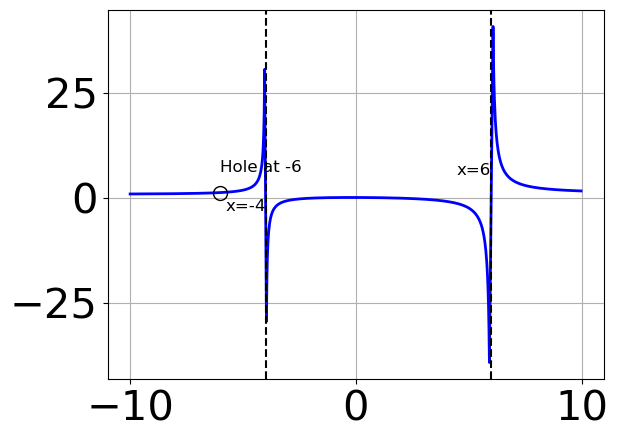
\includegraphics[width=0.5\textwidth]{../Figures/identifyGraphOfRationalFunctionC.png}
\end{center}
\begin{enumerate}[label=\Alph*.]
\item \( f(x)=\frac{x^{3} -2.0 x^{2} -4.0 x + 8.0}{x^{3} -4.0 x^{2} -36.0 x + 144.0} \)
\item \( f(x)=\frac{x^{3} -6.0 x^{2} -4.0 x + 24.0}{x^{3} -4.0 x^{2} -36.0 x + 144.0} \)
\item \( f(x)=\frac{x^{3} +6.0 x^{2} -4.0 x -24.0}{x^{3} +4.0 x^{2} -36.0 x -144.0} \)
\item \( f(x)=\frac{x^{3} +3.0 x^{2} -4.0 x -12.0}{x^{3} +4.0 x^{2} -36.0 x -144.0} \)
\item \( \text{None of the above are possible equations for the graph.} \)

\end{enumerate} }
\litem{
Determine the horizontal and/or oblique asymptotes in the rational function below.\[ f(x) = \frac{4x^{3} -8 x^{2} -25 x + 50}{2x^{2} -x -10} \]\begin{enumerate}[label=\Alph*.]
\item \( \text{Horizontal Asymptote of } y = 2.0  \)
\item \( \text{Horizontal Asymptote of } y = -2.0 \text{ and Oblique Asymptote of } y = 2x -3 \)
\item \( \text{Horizontal Asymptote of } y = 2.0 \text{ and Oblique Asymptote of } y = 2x -3 \)
\item \( \text{Oblique Asymptote of } y = 2x -3. \)
\item \( \text{Horizontal Asymptote at } y = -2.0 \)

\end{enumerate} }
\end{enumerate}

\end{document}